\section{Systemantworten}
Für die Analyse eines Systems kann eine Testfunktion herangezogen
werden. Hierzu wird dem System, welches sich im Gleichgewicht
befindet, eine definierte Eingabe eingespielt (Testfunktion) und
die Ausgangsgrösse beobachtet. Dies wird typisch für einzelne
Glieder oder Gruppen von glidern gemacht um deren 
Übertragungsfunktion zu prüfen.

Im Grunde genommen könnte jede Funktion als Testfunktion definiert
werden, jedoch gibt es vier Funktionen welche sich als besonders
nützlich erwiesen haben.
%
\begin{itemize}
	\item Stoss (Impuls)
    \item Sprung
    \item Rampe
    \item Sinus (harmonische Schwingung)
\end{itemize}
%
Nebst der harmonischen Schwingung haben alle diese Funktionen
einen Zusammenhang, denn sie sind jeweils die Ableitung bzw. das
Integral der anderen.

\begin{figure}[h!]
    \centering
    \begin{tikzpicture}[domain=0:2.5]
        % Koordinaten
        \coordinate (a1) at (0,0);
        \coordinate (b1) at ($ (a1) + (5,0) $);
        \coordinate (a2) at ($ (a1) + (0,3) $);
        \coordinate (b2) at ($ (a2) + (5,0) $);
        \coordinate (a3) at ($ (a2) + (0,3) $);
        \coordinate (b3) at ($ (a3) + (5,0) $);
        % Stoss
        \begin{scope}[shift={(a3)}]
            \draw[->] (-1,0) -- (3,0) node[below] {$t$};
            \draw[->] (0,-0.1) -- (0,2) node[left] {$x(t)$};
            \draw[thick, red] (-0.5,0) -- (2.5,0);
            \draw[thick, red, ->] (0,0) -- (0,1.5);
            \draw[red] (1,2) node[right] {$\delta(t) \,\laplace\,1$};
        \end{scope}
        % Stossantwort
        \begin{scope}[shift={(b3)}]
            \draw[->] (-1,0) -- (3,0) node[below] {$t$};
            \draw[->] (0,-0.1) -- (0,2) node[left] {$x(t)$};
            \draw[red, thick] (-0.5,0) -- (0,0);
            \draw[red, thick, samples=200] plot[id=B3]
                function{sin(x*5)*exp(-2*x)*3};
            \draw[red] (1,2) node[right] {$g(t) \,\laplace\, G(s)$}; 
        \end{scope}
        % Sprung
        \begin{scope}[shift={(a2)}]
            \draw[->] (-1,0) -- (3,0) node[below] {$t$};
            \draw[->] (0,-0.1) -- (0,2) node[left] {$x(t)$};
            \draw[thick, red] (-0.5,0) -- (0,0) -- (0,1) -- (2.5,1);
            \draw[red] (1,2) node[right] {$\sigma(t) \,\laplace\, s$};
        \end{scope}
        % Sprungantwort
        \begin{scope}[shift={(b2)}]
            \draw[thin, gray] (-0.5,0) -- (0,0) -- (0,1) -- (2.5,1);
            \draw[->] (-1,0) -- (3,0) node[below] {$t$};
            \draw[->] (0,-0.1) -- (0,2) node[left] {$x(t)$};
            \draw[red, thick] (-0.5,0) -- (0,0);
            \draw[red, thick, samples=200] plot[id=B2]
                function{-0.5*2*exp(-2*x)*(sin(x*10)+cos(x*10))+1};
            \draw[red] (1,2) node[right] 
                {$h(t) \,\laplace\, H(s) 
                    = \displaystyle \frac{1}{s} \cdot G(s)$};
        \end{scope}
        % Rampe
        \begin{scope}[shift={(a1)}]
            \draw[->] (-1,0) -- (3,0) node[below] {$t$};
            \draw[->] (0,-0.1) -- (0,2) node[left] {$x(t)$};
            \draw[thick, red] (-0.5,0) -- (0,0) -- (2.5,1.5);
            \draw[red] (1,2) node[right] 
                {$t \cdot \sigma(t) \,\laplace\, \frac{1}{s^2}$};
        \end{scope}
        % Rampenantwort
        \begin{scope}[shift={(b1)}]
            \draw[thin, gray] (-0.5,0) -- (0,0) -- (2.5,1.5);
            \draw[->] (-1,0) -- (3,0) node[below] {$t$};
            \draw[->] (0,-0.1) -- (0,2) node[left] {$x(t)$};
            \draw[thick, red] (-0.5,0) -- (0,0);
            \draw[red, thick, samples=200] plot[id=B1]
                function{0.6*(x+0.5*exp(-2*x)*cos(10*x)-0.5)};
            \draw[red] (1,2) node[right] 
                {$r(t) \,\laplace\, R(s) 
                    = \displaystyle \frac{1}{s^2} \cdot G(s)$};
        \end{scope}
    \end{tikzpicture}
\end{figure}

\subsection{Sprungantwort}
Als Sprungantwort wird der Verlauf der Ausgangsgrösse eines
Übertragungsgliedes oder Systems bezeichnet, welches ausgehend
vom Gleichgewichtszustand eine Sprungfunktion am Eingang 
erfahren hat.
%
\begin{figure}[h!]
    \centering
    \begin{tikzpicture}
        \draw[->] (-1,0) -- (3,0) node[below] {$t$};
        \draw[->] (0,-0.1) -- (0,2) node[left] {$x(t)$};
        \draw[thick, red] 
            (-0.5,0) -- (0,0) -- (0,1) -- (2.5,1);
        \draw[] (0,0) node[below] {$0$};
        \draw[] (0.1,1) -- (-0.1,1) node[left] {$\hat{x}$}; 
    \end{tikzpicture} 
    %
    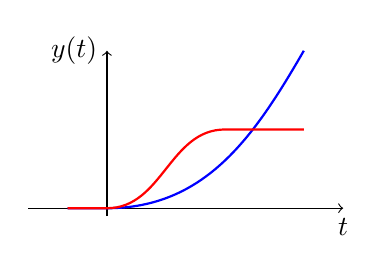
\begin{tikzpicture}
        \draw[->] (-1,0) -- (3,0) node[below] {$t$};
        \draw[->] (0,-0.1) -- (0,2) node[left] {$y(t)$};
        \draw[thick, blue] (-0.5,0) -- (0,0)
            to[out=0,in=-120] (2.5,2);
        \draw[thick, red] (-0.5,0) -- (0,0) 
            to[out=0,in=180] (1.5,1) -- (2.5,1);
    \end{tikzpicture}
\end{figure}
%
Solch eine Sprungantwort zeigt z.B. auf, ob ein Übertragungsglied
stabil ist (konvergiert) oder nicht (divergiert). Es können aber
weitere Informationen aus der Sprungantwort entnommen werden wie
etwa das zu Grunde liegende Übertragiungsverhalten und die 
zugehörigen Parameter.

\subsubsection{Identifikation}
Es gibt einige Charakteristiken in der Sprungantwort, welche ein
Übertragungsglied mehr oder weniger eindeutig identifizieren lassen.

\begin{itemize}
    \item Gibt es eine Schwingung in der Sprungantwort, dann muss es 
        ein Glied zweiter oder höherer Ordnung sein.
    \item Ist die Steigung der Sprungantwort bei $t=0$ gleich $0$, dann
        muss es eine Verzögerung im Glied haben.
    \item Divergiert die Sprungantwort, dann muss es mindestens einen
        Integrator im Glied haben. 
    \item Ist die Steigung der Sprungantwort bei $t=0$ unendlich, dann
        muss es einen Differenzierer im Glied haben.
    \item Konvergiert der Endwert der Sprungantwort zu null, dann muss
        es einen Differenzierer im Glied haben.
\end{itemize}

\subsection{Impulsantwort}
Analog zur Sprungantwort liefert die Impulsantwort eine Charakterisierung
eines Übertragungsglides. Die besondere Eigenschaft des Impulses ist,
dass aufgrund der unendlichen Steigung des Stosses, ein unendlich weites
Frequenzspektrum vorliegt. Der Ideale Impuls, also der Dirac-Stoss, kann
jedoch nur in der Theorie erzeugt werden, weshalb die Sprungantwort
eine übergeordnete Rolle spielt in der Praxis.
%
\begin{figure}[h!]
    \centering
    \begin{tikzpicture}
        \draw[->] (-1,0) -- (3,0) node[below] {$t$};
        \draw[->] (0,-0.1) -- (0,2) node[left] {$x(t)$};
        \draw[thick, red] (-0.5,0) -- (2.5,0);
        \draw[thick, red, ->] (0,0) -- (0,1.5); 
    \end{tikzpicture} 
    %
    \begin{tikzpicture}[domain=0:2.5]
        \draw[->] (-1,0) -- (3,0) node[below] {$t$};
        \draw[->] (0,-0.1) -- (0,2) node[left] {$y(t)$};
        \draw[red, thick] (-0.5,0) -- (0,0);
        \draw[red, thick] (0,0) -- (0,1.5);
        \draw[red, thick, samples=200] plot[id=dirac]
            function{1.5*exp(-2*x)};
        \draw[blue, thick, samples=200] plot[id=B3]
            function{sin(1.2*x)*exp(-1.2*x)*3};
        \draw[red, thick, samples=200] plot[id=dirac]
            function{1.5*exp(-2*x)};
    \end{tikzpicture}
\end{figure}

